\documentclass{article}
\usepackage{graphicx}
\usepackage{url}
\usepackage[colorlinks, linkcolor=black, citecolor=black]{hyperref}
\hypersetup{urlcolor=blue}
\usepackage{minted}
\usepackage{subcaption}
\usepackage[margin=1in]{geometry}

\title{CSIGen Documentation}
\author{Berkay Guler}
\date{Last Updated: April 2nd, 2026}


\begin{document}

\maketitle

\clearpage

\section{Scene File Generation}
The Geo2SigMap package provides scripts to extract an XML file containing scene information (buildings and ground terrain) from selected bounding box coordinates.

\flushleft
For example, the following command generates the file for the specified bounding box.

\begin{verbatim}
    scenegen bbox -71.0602 42.3512 -71.0484 42.3591 --data-dir
    scenes/sample_scene --enable-lidar-terrain
\end{verbatim}

Note: \href{https://bboxfinder.com}{bboxfinder.com} is a simple website for obtaining the bounding box coordinates of a desired region. It can also be used to visualize a bounding box, given its coordinates.

If the \texttt{--enable-lidar-terrain} flag is not passed, the generated scene does not have elevation information, and a simple horizontal plane is used as the ground terrain.

The generated scene files are saved under the \texttt{--data-dir} folder, with the \texttt{scene.xml} file containing references to mesh objects stored as \texttt{.ply} files under the \texttt{mesh} subfolder. Load the scene using \texttt{load\_scene(scene.xml, merge\_shapes=False)}. Setting \texttt{merge\_shapes=True} prevents objects from loading properly.

\vspace{1em}

After loading the scene, access objects using \texttt{scene.objects["object\_name"]}. Three objects are particularly important:
\begin{itemize}
  \item \texttt{building\_x\_rooftop}: Rooftop object of the $x$th building
  \item \texttt{building\_x\_wall}: Wall object of the $x$th building
  \item \texttt{ground}: The terrain object from \texttt{lidar\_terrain.ply}
\end{itemize}

Scene metadata (longitude/latitude bounding box values) is also stored in \texttt{scene.xml}.

\clearpage

\section{Channel Generation}
This framework enables generation of large-scale channel state information (CSI) datasets with customizable simulation parameters via the following configuration file.

\begin{minted}[
  frame=single,
  framesep=1mm,
  baselinestretch=1,
  bgcolor=lightgray!20,
  linenos,
  breaklines=true,
  fontsize=\footnotesize,
  label=config.yaml
]{yaml}
# Example configuration for channel generation

# Scene configuration
scene_xml_path: "./scenes/boston_1/scene.xml"  # Path to the 3D scene XML file generated by scenegen
carrier_frequency: 3500000000.0  # Carrier frequency in Hz

# Scene setup parameters
scene_center: [0.0, 0.0]  # 2D coordinate [x, y] specifying scene center in meters
antenna_height_offset: 10.0  # Vertical offset of base station antennas above rooftops (meters)
num_deployment_buildings: 1  # Number of buildings for base station deployment
clip_terrain_to_buildings: true  # Whether to clip terrain mesh to building boundaries
terrain_clip_margin: 15.0  # Margin around buildings when clipping (meters)
user_shift_from_ground: 1.5  # UE height above ground (meters)
# override_ground_material: "concrete"  # optional: assign ITU concrete to ground (omit key if unused)

# TX antenna array parameters
tx_num_rows: 4  # Array dimensions (rows)
tx_num_cols: 8  # Array dimensions (columns)
tx_vertical_spacing: 0.5  # Element spacing in wavelengths (vertical)
tx_horizontal_spacing: 0.5  # Element spacing in wavelengths (horizontal)
tx_pattern: "tr38901"  # Radiation pattern: tr38901 (3GPP), dipole, iso, or hw_dipole
tx_polarization: "V"  # Polarization: cross (±45°), V, H, or VH

# RX antenna array parameters
rx_num_rows: 1  # Array dimensions (rows)
rx_num_cols: 1  # Array dimensions (columns)
rx_vertical_spacing: 0.5  # Element spacing in wavelengths (vertical)
rx_horizontal_spacing: 0.5  # Element spacing in wavelengths (horizontal)
rx_pattern: "iso"  # Radiation pattern: tr38901 (3GPP), dipole, iso, or hw_dipole
rx_polarization: "V"  # Polarization: cross (±45°), V, H, or VH

# Base station parameters
num_sectors: 6  # Sectors per base station (azimuth angles computed automatically for uniform coverage)
mechanical_tilt: 10.0  # Antenna downtilt angle (degrees)
azimuth_offset: 0.0  # Global azimuth rotation (degrees)
tx_power_dbm: 43.0  # Transmit power per array (dBm)

# Radio map solver parameters
radio_map_specular_reflection: true  # Mirror-like reflections
radio_map_diffuse_reflection: true  # Scattering from rough surfaces
radio_map_refraction: true  # Transmission through materials (Snell's law)
radio_map_diffraction: true  # Signal bending around obstacles
radio_map_edge_diffraction: true  # Diffraction at edges
radio_map_diffraction_lit_region: false  # Diffraction in LoS regions
radio_map_max_depth: 5  # Maximum ray-scene interactions per path
radio_map_samples_per_tx: 1000000  # Number of samples per TX antenna array (10^6)
radio_map_seed: 1  # Seed for radio map solver (reproducibility)

# User sampling parameters
num_user_samples_per_tx: 200  # Users sampled per TX array
user_sample_seed: 1  # Random seed for reproducibility
user_sample_min_val_db: -150  # Coverage thresholds (dB) - minimum
user_sample_max_val_db: 100  # Coverage thresholds (dB) - maximum
user_sample_min_dist: 0.0  # Distance constraints (meters) - minimum
user_sample_max_dist: 10000.0  # Distance constraints (meters) - maximum
user_sample_metric: "path_gain"  # Sampling metric: path_gain, rss, or sinr
tx_association: true  # Associate users with strongest-signal TX
sample_center_pos: true  # Sample from cell centers (deterministic) vs. randomly within cells
scene_edge_epsilon: 1.0  # Minimum distance in meters from measurement surface edges to keep users (0.0 means no filtering)

# Mobility preset
mobility_preset: "vehicular"  # Select preset to use (must be a key in mobility_presets)

# User equipment mobility presets
mobility_presets:
  stationary:
    orientation_mode: "random"  # random or to_tx (pointing toward serving TX)
    speed_distribution: null  # null (stationary), pedestrian (0.5--2 m/s), vehicular (8--30 m/s), or uniform_continuous with custom speed_min/speed_max
  stationary_to_tx:
    orientation_mode: "to_tx"  # random or to_tx (pointing toward serving TX)
    speed_distribution: null  # null (stationary), pedestrian (0.5--2 m/s), vehicular (8--30 m/s), or uniform_continuous with custom speed_min/speed_max
  pedestrian:
    orientation_mode: "random"  # random or to_tx (pointing toward serving TX)
    speed_distribution: "pedestrian"  # null (stationary), pedestrian (0.5--2 m/s), vehicular (8--30 m/s), or uniform_continuous with custom speed_min/speed_max
    direction_mode: "random"  # Movement direction (random)
  pedestrian_to_tx:
    orientation_mode: "to_tx"  # random or to_tx (pointing toward serving TX)
    speed_distribution: "pedestrian"  # null (stationary), pedestrian (0.5--2 m/s), vehicular (8--30 m/s), or uniform_continuous with custom speed_min/speed_max
    direction_mode: "random"  # Movement direction (random)
  vehicular:
    orientation_mode: "random"  # random or to_tx (pointing toward serving TX)
    speed_distribution: "vehicular"  # null (stationary), pedestrian (0.5--2 m/s), vehicular (8--30 m/s), or uniform_continuous with custom speed_min/speed_max
    direction_mode: "random"  # Movement direction (random)
  slow_walking:
    orientation_mode: "random"  # random or to_tx (pointing toward serving TX)
    speed_distribution: "uniform_continuous"  # null (stationary), pedestrian (0.5--2 m/s), vehicular (8--30 m/s), or uniform_continuous with custom speed_min/speed_max
    speed_min: 0.5  # in m/s
    speed_max: 1.5  # in m/s
    direction_mode: "random"  # Movement direction (random)
  fast_walking:
    orientation_mode: "random"  # random or to_tx (pointing toward serving TX)
    speed_distribution: "uniform_continuous"  # null (stationary), pedestrian (0.5--2 m/s), vehicular (8--30 m/s), or uniform_continuous with custom speed_min/speed_max
    speed_min: 1.5  # in m/s
    speed_max: 2.5  # in m/s
    direction_mode: "random"  # Movement direction (random)

# Path solver parameters
path_solver_max_depth: 5  # Maximum ray-scene interactions per path
path_solver_max_num_paths_per_src: 10000000  # Maximum paths per source (10^7)
path_solver_samples_per_src: 10000000  # Ray samples per source (10^7)
path_solver_synthetic_array: true  # Use synthetic array approximation for efficiency
path_solver_los_mode: true  # Include line-of-sight paths
path_solver_specular_reflection: true  # Mirror-like reflections
path_solver_diffuse_reflection: true  # Scattering from rough surfaces
path_solver_refraction: true  # Transmission through materials (Snell's law)
path_solver_diffraction: true  # Signal bending around obstacles
path_solver_edge_diffraction: true  # Diffraction at edges
path_solver_diffraction_lit_region: false  # Diffraction in LoS regions
path_solver_seed: 1  # Random seed
path_solver_per_tx_users_only: false  # Compute paths only for TX-associated users

# OFDM parameters
num_subcarriers: 32  # OFDM subcarrier count
num_ofdm_symbols: 14  # Time-domain symbols
subcarrier_spacing: 30000.0  # Spacing in Hz

# Channel Frequency Response (CFR) parameters
cfr_normalize_delays: false  # Normalize delays relative to first path
cfr_normalize: false  # Normalize CFR magnitude
cfr_out_type: "numpy"  # Output backend
\end{minted}

\subsection{Configuration Reference}

\subsubsection{Scene Configuration}
\begin{itemize}
  \item \texttt{scene\_xml\_path}: Path to the 3D scene XML file generated by \texttt{scenegen}.
  \item \texttt{carrier\_frequency}: Carrier frequency in Hz.
\end{itemize}

\subsubsection{Scene Setup Parameters}
\begin{itemize}
  \item \texttt{scene\_center}: 2D coordinate $[x, y]$ specifying scene center in meters.
  \item \texttt{antenna\_height\_offset}: Vertical offset of base station antennas above rooftops (meters).
  \item \texttt{num\_deployment\_buildings}: Number of buildings for base station deployment.
  \item \texttt{clip\_terrain\_to\_buildings}: Whether to clip terrain mesh to building boundaries.
  \item \texttt{terrain\_clip\_margin}: Margin around buildings when clipping (meters).
  \item \texttt{user\_shift\_from\_ground}: UE height above ground (meters).
  \item \texttt{override\_ground\_material} (optional): If set to \texttt{"concrete"}, the scene's \texttt{ground} object is assigned an ITU concrete radio material. Omit the key or leave unset to keep scene XML materials unchanged.
\end{itemize}

\subsubsection{Antenna Array Parameters (TX and RX)}
\begin{itemize}
  \item \texttt{tx\_num\_rows}, \texttt{tx\_num\_cols} / \texttt{rx\_num\_rows}, \texttt{rx\_num\_cols}: Array dimensions.
  \item \texttt{tx\_vertical\_spacing}, \texttt{tx\_horizontal\_spacing} / \texttt{rx\_vertical\_spacing}, \texttt{rx\_horizontal\_spacing}: Element spacing in carrier wavelengths.
  \item \texttt{tx\_pattern}, \texttt{rx\_pattern}: Radiation pattern---\texttt{tr38901} (3GPP), \texttt{dipole}, \texttt{iso}, or \texttt{hw\_dipole}.
  \item \texttt{tx\_polarization}, \texttt{rx\_polarization}: \texttt{cross} ($\pm 45^{\circ}$), \texttt{V}, \texttt{H}, or \texttt{VH}.
\end{itemize}

\subsubsection{Base Station Parameters}
\begin{itemize}
  \item \texttt{num\_sectors}: Sectors per base station (azimuth angles computed automatically for uniform coverage).
  \item \texttt{mechanical\_tilt}: Antenna downtilt angle (degrees).
  \item \texttt{azimuth\_offset}: Global azimuth rotation (degrees).
  \item \texttt{tx\_power\_dbm}: Transmit power per array (dBm).
\end{itemize}

\subsubsection{Ray Tracing Parameters (Radio Map and Path Solver)}
\label{subsec:ray-tracing-radio-path}
These control ray-scene interactions for both the radio map and the path solver. The same physical toggles appear twice in YAML: each boolean is prefixed \texttt{radio\_map\_} for \texttt{RadioMapSolver} and \texttt{path\_solver\_} for \texttt{PathSolver}, so the two stages can be configured independently (e.g., fewer interactions or samples for the map, more for detailed paths). See \href{https://arxiv.org/pdf/2504.21719}{Sionna RT: Technical Report} for interaction semantics.
\begin{itemize}
  \item \texttt{radio\_map\_max\_depth}, \texttt{path\_solver\_max\_depth}: Maximum ray-scene interactions per path.
  \item \texttt{radio\_map\_samples\_per\_tx}: Number of samples per TX for radio map (e.g., $10^6$).
  \item \texttt{radio\_map\_seed}: Seed for radio map solver (reproducibility).
  \item \texttt{path\_solver\_max\_num\_paths\_per\_src}, \texttt{path\_solver\_samples\_per\_src}: Max paths and ray samples per source (e.g., $10^7$).
  \item \texttt{radio\_map\_specular\_reflection}, \texttt{path\_solver\_specular\_reflection} (and \texttt{\ldots diffuse\_reflection}): Mirror-like and rough-surface scattering.
  \item \texttt{radio\_map\_refraction}, \texttt{path\_solver\_refraction}: Transmission through materials (Snell's law).
  \item \texttt{radio\_map\_diffraction}, \texttt{path\_solver\_diffraction}; \texttt{radio\_map\_edge\_diffraction}, \texttt{path\_solver\_edge\_diffraction}: Signal bending and edge diffraction.
  \item \texttt{radio\_map\_diffraction\_lit\_region}, \texttt{path\_solver\_diffraction\_lit\_region}: Diffraction in LoS regions.
\end{itemize}

\subsubsection{User Sampling Parameters}
\begin{itemize}
  \item \texttt{num\_user\_samples\_per\_tx}: Users sampled per TX array.
  \item \texttt{user\_sample\_seed}: Random seed for reproducibility.
  \item \texttt{user\_sample\_min/max\_val\_db}: Coverage thresholds (dB).
  \item \texttt{user\_sample\_min/max\_dist}: Distance constraints (meters).
  \item \texttt{user\_sample\_metric}: Sampling metric---\texttt{path\_gain}, \texttt{rss}, or \texttt{sinr}.
  \item \texttt{tx\_association}: If \texttt{true}, sampled positions are restricted to cells where the chosen metric is strongest for that transmitter; if \texttt{false}, a cell may be kept for one TX even if another TX would yield a higher metric at that location.
  \item \texttt{sample\_center\_pos}: If \texttt{true}, positions lie on radio-map cell centers (grid); if \texttt{false}, positions are drawn at random within each cell surface.
  \item \texttt{scene\_edge\_epsilon}: Minimum distance in meters from measurement surface outer edges to keep users. Users within this distance from any outer edge are filtered out. Set to 0.0 to disable filtering.
\end{itemize}

\subsubsection{Mobility Presets}
The top-level key \texttt{mobility\_preset} must name one entry in the \texttt{mobility\_presets} mapping. Each preset specifies:
\begin{itemize}
  \item \texttt{orientation\_mode}: \texttt{random} or \texttt{to\_tx} (pointing toward serving TX).
  \item \texttt{speed\_distribution}: \texttt{null} (stationary), \texttt{pedestrian} (0.5--2 m/s), \texttt{vehicular} (8--30 m/s), or \texttt{uniform\_continuous} with custom \texttt{speed\_min}/\texttt{speed\_max}.
  \item \texttt{direction\_mode}: Movement direction (\texttt{random}), required when the preset uses a non-null speed distribution.
\end{itemize}

\subsubsection{Path Solver Parameters}
Beyond the knobs listed here, path solving also uses \texttt{path\_solver\_max\_depth} and the \texttt{path\_solver\_*} interaction toggles (specular reflection, diffuse reflection, refraction, diffraction, edge diffraction, diffraction-lit region). Those mirror the \texttt{radio\_map\_*} keys so the solver and radio map can diverge independently; see~\S~\ref{subsec:ray-tracing-radio-path}.
\begin{itemize}
  \item \texttt{path\_solver\_max\_num\_paths\_per\_src}: Maximum paths per source.
  \item \texttt{path\_solver\_samples\_per\_src}: Ray samples per source.
  \item \texttt{path\_solver\_synthetic\_array}: Use synthetic array approximation for efficiency.
  \item \texttt{path\_solver\_los\_mode}: Include line-of-sight paths.
  \item \texttt{path\_solver\_seed}: Random seed.
  \item \texttt{path\_solver\_per\_tx\_users\_only}: Compute paths only for TX-associated users.
\end{itemize}

\subsubsection{OFDM and CFR Parameters}
\begin{itemize}
  \item \texttt{num\_subcarriers}: OFDM subcarrier count.
  \item \texttt{num\_ofdm\_symbols}: Time-domain symbols.
  \item \texttt{subcarrier\_spacing}: Spacing in Hz.
  \item \texttt{cfr\_normalize\_delays}: Normalize delays relative to first path.
  \item \texttt{cfr\_normalize}: Normalize CFR magnitude.
  \item \texttt{cfr\_out\_type}: Output tensor backend token (YAML string). Allowed values mirror \texttt{src.config\_validator}: \texttt{numpy}, \texttt{tf} (TensorFlow), \texttt{torch}, \texttt{jax}, \texttt{drjit}.
\end{itemize}

\clearpage
\section{Framework Architecture}

The generation pipeline transforms a configuration file into channel frequency response (CFR) data through these sequential steps:

\begin{enumerate}
  \item \textbf{Scene Setup}: Load 3D geometry, extract building info, optionally clip terrain, determine antenna positions.
  \item \textbf{Antenna Configuration}: Configure shared TX/RX array properties.
  \item \textbf{Base Station Deployment}: Deploy multi-sector base stations with uniform azimuthal coverage.
  \item \textbf{Radio Map Computation}: Generate coverage maps via ray tracing.
  \item \textbf{User Sampling}: Sample UE positions based on coverage, distance, and association constraints.
  \item \textbf{Edge Filtering}: Optionally filter users too close to measurement surface edges (if \texttt{scene\_edge\_epsilon} $> 0$).
  \item \textbf{Receiver Creation}: Create receivers with mobility parameters.
  \item \textbf{Path Solving}: Compute ray-traced paths per TX.
  \item \textbf{CFR Computation}: Convert paths to frequency response arrays (one tensor per TX over all receivers considered for that TX).
  \item \textbf{Valid-Path Filtering and LoS/NLOS Labels}: After CFR is built, path delays and Sionna interaction types are evaluated in a single pass (\texttt{\_compute\_rx\_valid\_and\_los\_masks}). Receivers without any path with strictly positive delay ($\tau > 0$) are invalid and dropped. For each remaining (valid) channel, a binary line-of-sight flag is set: \texttt{1} if at least one valid path is pure LoS (all ray--scene interactions along that path are \texttt{InteractionType.NONE}), and \texttt{0} if all valid paths involve at least one non-trivial interaction (NLoS). The saved CFR tensor, \texttt{rx\_positions}, and \texttt{rx\_names} are sliced to valid channels only. Per-TX metadata includes the transmit antenna position (\texttt{tx\_position}), receive positions for valid channels (\texttt{rx\_positions}), corresponding receiver names (\texttt{rx\_names}), \texttt{num\_valid\_channels}, and \texttt{los\_binary} (length equal to the number of valid channels, aligned with the CFR user axis).
\end{enumerate}

\subsection{Key Design Choices}

\subsubsection{Shared Antenna Arrays}
Sionna RT enforces a single TX and RX antenna configuration per scene. All base stations share identical TX array properties; all UEs share identical RX properties.

\subsubsection{Per-Transmitter Path Solving}
Paths are solved separately per TX rather than simultaneously for all TX-RX pairs. This reduces complexity from $O(N \times M)$ to $O(M)$ per TX. With TX association enabled, each TX processes only its associated users, reducing computation to $O(\texttt{num\_users\_per\_tx})$ per TX. This enables scaling to scenarios infeasible with simultaneous solving.

\subsubsection{Antenna Placement}
Base stations deploy on the highest buildings (sorted by rooftop height). For each building, the antenna is placed at the rooftop vertex closest to the scene center, minimizing self-shadowing by positioning the building mass behind the antenna relative to the primary coverage area.

\subsubsection{Measurement Surface}
The framework creates a measurement surface by shifting the terrain mesh vertically by \texttt{user\_shift\_from\_ground}. If terrain clipping is enabled, it occurs before this shift.

\subsubsection{Configuration Validation}
All parameters are validated before generation, catching errors early with clear messages. Use \texttt{load\_validated\_config(path)} (from \texttt{src.config\_validator}) to load a YAML file into a dictionary suitable for the generator API.

\subsubsection{Python API and Saved Outputs}
Channel generation is exposed as \texttt{generate\_channels(config)} in \texttt{src.channel\_generator}: it is a \emph{streaming} iterator that yields one dictionary per transmit sector index, in order, without holding all TX CFR tensors in memory at once. Each yielded item has keys \texttt{tx\_idx}, \texttt{tx\_name}, \texttt{h\_tx} (NumPy CFR for valid channels only), and \texttt{tx\_metadata} (positions, names, LoS flags, counts, embedded \texttt{config} copy, CFR shape/dtype, etc.).

The helper \texttt{save\_channel\_data} (\texttt{src.channel}) writes a compressed \texttt{.npz} per TX containing array \texttt{h}, \texttt{shape}, \texttt{dtype}, and a nested \texttt{metadata} object. The script \texttt{scripts/run.py} loads a config, iterates \texttt{generate\_channels}, saves one file per TX under a timestamped output directory, and writes a run-level \texttt{metadata.yaml} summary (scene name, timestamp, global user counts, per-TX CFR shapes/dtypes, full config).

\clearpage
\section{Sample Flow}

\subsection{Scene Setup and Antenna Deployment}

To avoid sampling users outside the urban area, terrain can be clipped at scene edges (Fig.~\ref{fig:scene_clip}). The highest \texttt{num\_deployment\_buildings} are selected for base station deployment (Fig.~\ref{fig:antenna_placement}).

\begin{figure}[htbp]
  \centering
  \begin{subfigure}{0.45\textwidth}
    \centering
    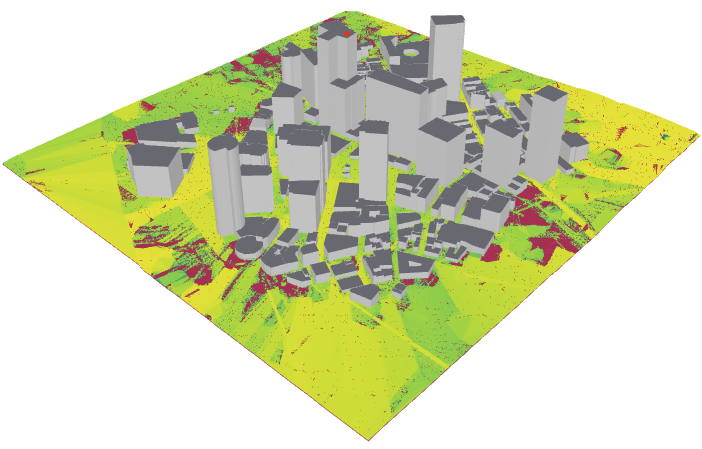
\includegraphics[width=\textwidth]{figures/scene_1.png}
    \caption{Before clipping}
  \end{subfigure}
  \hfill
  \begin{subfigure}{0.45\textwidth}
    \centering
    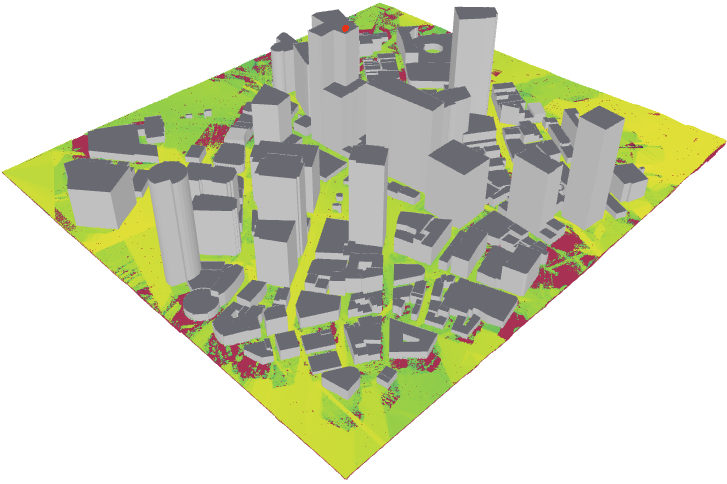
\includegraphics[width=\textwidth]{figures/scene_1_clipped.png}
    \caption{After clipping (15\,m margin)}
  \end{subfigure}
  \caption{Effect of Terrain Clipping}
  \label{fig:scene_clip}
\end{figure}

\begin{figure}
  \centering
  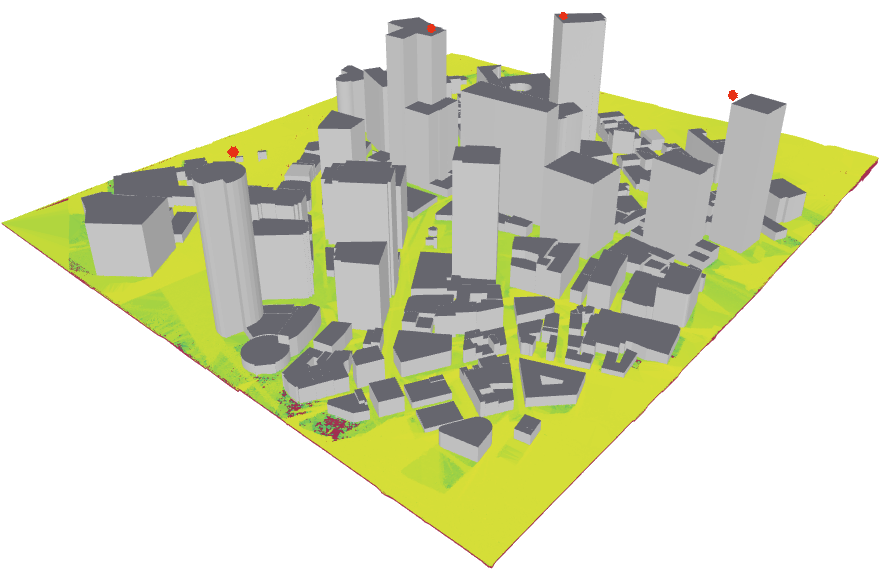
\includegraphics[width=0.5\linewidth]{figures/antenna_placement.png}
  \caption{Base station deployment with \texttt{num\_deployment\_buildings=4} (red dots)}
  \label{fig:antenna_placement}
\end{figure}

\subsection{Base Station Configuration}

Each base station is deployed with \texttt{num\_sectors} sectors at automatically computed azimuth angles for uniform coverage (e.g., 0°, 120°, 240° for 3 sectors). Sectors share position but differ in orientation.

\subsection{Radio Map and User Sampling}

The radio map computes signal strength across the measurement surface using shooting-and-bouncing-rays (SBR). User positions are sampled based on:
\begin{itemize}
  \item Coverage thresholds (min/max signal strength)
  \item Distance constraints (min/max from TX)
  \item TX association (optional strongest-signal pairing)
  \item Sampling mode (cell centers or random within cells)
\end{itemize}

See Fig.~\ref{fig:user_sampling} for an example with 5 base stations, 3 sectors each, and 100 users per TX.

\begin{figure}
  \centering
  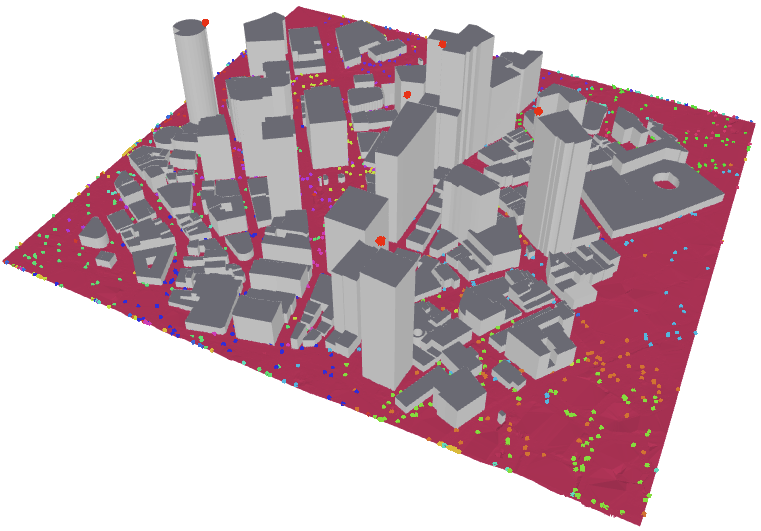
\includegraphics[width=0.5\linewidth]{figures/scene_1_user_sample.png}
  \caption{User sampling: 5 BSs $\times$ 3 sectors, 100 users/TX (colored points)}
  \label{fig:user_sampling}
\end{figure}

\subsection{Receiver Creation and Mobility}

Receivers are created with mobility parameters from the selected preset. Orientation can be random or toward the serving TX. Velocity is sampled from the specified distribution with random direction.

\subsection{Edge Filtering}

After user sampling, positions can be filtered to remove users too close to the measurement surface outer edges. This is controlled by the \texttt{scene\_edge\_epsilon} parameter. The effect of this parameter is visualized in Fig.~\ref{fig:edge_user_filter}. Note that edge filtering is applied as a filter-out mechanism after user sampling. Therefore, it may change the number of effective users drastically especially if this parameter has a large value.  


\begin{figure}[h]
  \centering
  \begin{subfigure}{0.45\textwidth}
    \centering
    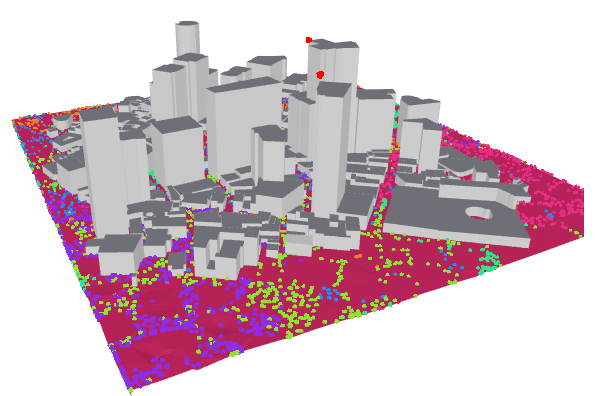
\includegraphics[width=\textwidth]{figures/no_edge_filter.png}
    \caption{\texttt{scene\_edge\_epsilon=0}}
  \end{subfigure}
  \hfill
  \begin{subfigure}{0.45\textwidth}
    \centering
    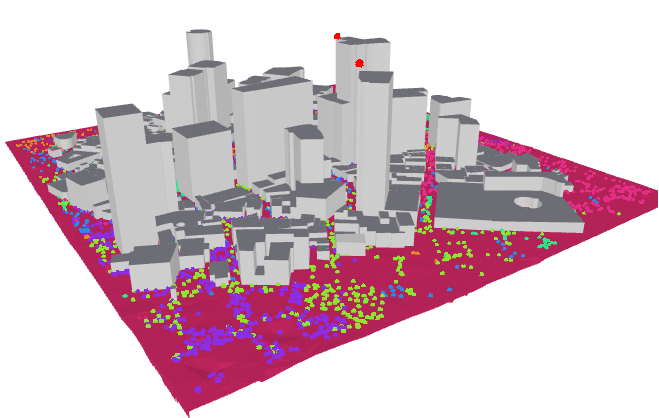
\includegraphics[width=\textwidth]{figures/edge_filter_15meters.png}
    \caption{\texttt{scene\_edge\_epsilon=15} meters}
  \end{subfigure}
  \caption{Filtering out users close to outer edges of the scene. Here \texttt{num\_sectors = 3}, \texttt{num\_deployment\_buildings = 2}, and \texttt{num\_user\_samples\_per\_tx = 1000}}
  \label{fig:edge_user_filter}
\end{figure}

\subsection{Valid-Path Filtering and LoS/NLOS Labels}

After path solving and CFR computation, the pipeline evaluates validity and LoS/NLOS jointly from the \texttt{Paths} object: path delays ($\tau > 0$) and per-path interaction records (Sionna \texttt{interactions}) determine which receivers have any valid path and whether a valid channel has at least one pure LoS path (no reflections, diffraction, etc.). Receivers with no valid paths are dropped; CFR arrays and aligned metadata (\texttt{rx\_positions}, \texttt{rx\_names}) are restricted to the valid subset. Per-TX metadata also stores the serving sector antenna position as \texttt{tx\_position}. The field \texttt{num\_valid\_channels} gives the count of valid channels, and \texttt{los\_binary} is a length-\texttt{num\_valid\_channels} array with \texttt{1} for LoS and \texttt{0} for NLoS, in the same order as rows of the filtered CFR. We include a histogram of number of paths from a TX to all sampled users displayed in Fig.~\ref{fig:num_paths}.

\begin{figure}[h]
  \centering
  \begin{subfigure}{0.49\textwidth}
    \centering
    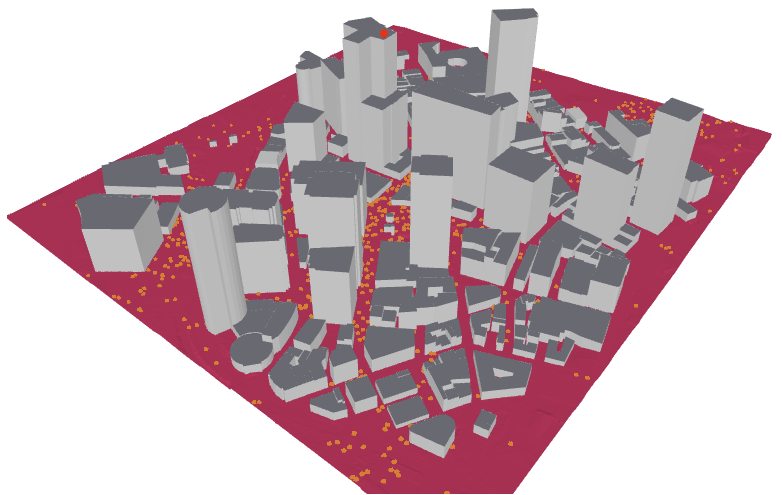
\includegraphics[width=\textwidth]{figures/boston_path_histogram_a.png}
    \caption{The TX antenna (red) and sampled users (brown) in Boston}
  \end{subfigure}
  \hfill
  \begin{subfigure}{0.49\textwidth}
    \centering
    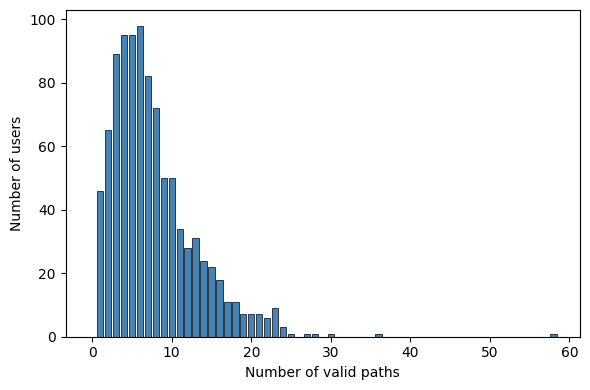
\includegraphics[width=\textwidth]{figures/boston_path_hist_b.png}
    \caption{Histogram of valid paths}
  \end{subfigure}
  \caption{Distribution of number of paths after removing invalid users}
  \label{fig:num_paths}
\end{figure}

\subsection{Channel Frequency Response}
After the paths are computed from a TX to a set of RXs, the channel frequency response can be derived from the path gains and delays. For \texttt{mobility\_preset="vehicular"}, \texttt{num\_subcarriers=32}, \texttt{tx\_num\_rows=1}, \texttt{tx\_num\_cols=32}, \texttt{rx\_num\_rows=1}, \texttt{rx\_num\_cols=1}, \texttt{num\_ofdm\_symbols=14}, and \texttt{subcarrier\_spacing=30}\,KHz, we include the time-frequency response for a fixed TX antenna index in Fig.~\ref{fig:cfr} and TX antenna-frequency response for a fixed OFDM symbol in Fig.~\ref{fig:afr}.

\begin{figure}
    \centering
    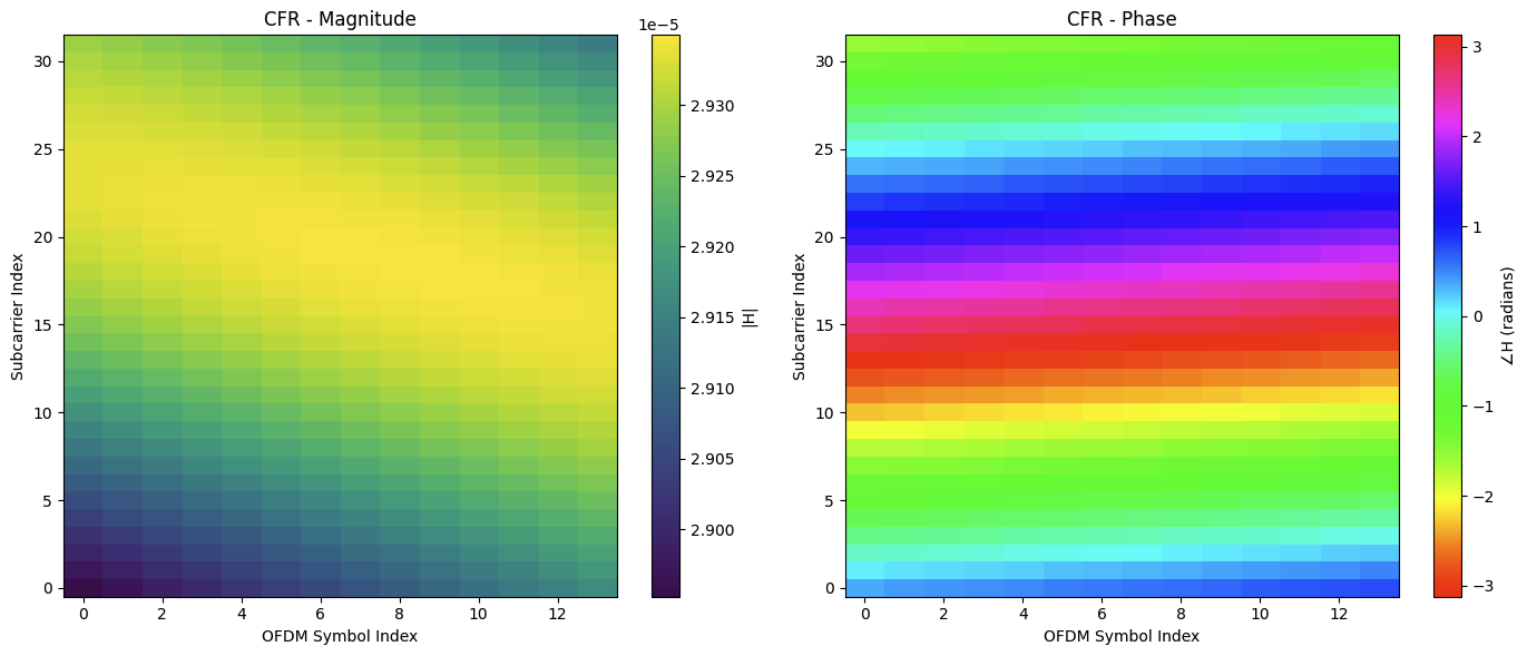
\includegraphics[width=0.9\linewidth]{figures/cfr.png}
    \caption{Time-frequency response (magnitude on the left, phase on the right)}
    \label{fig:cfr}
\end{figure}

\begin{figure}
    \centering
    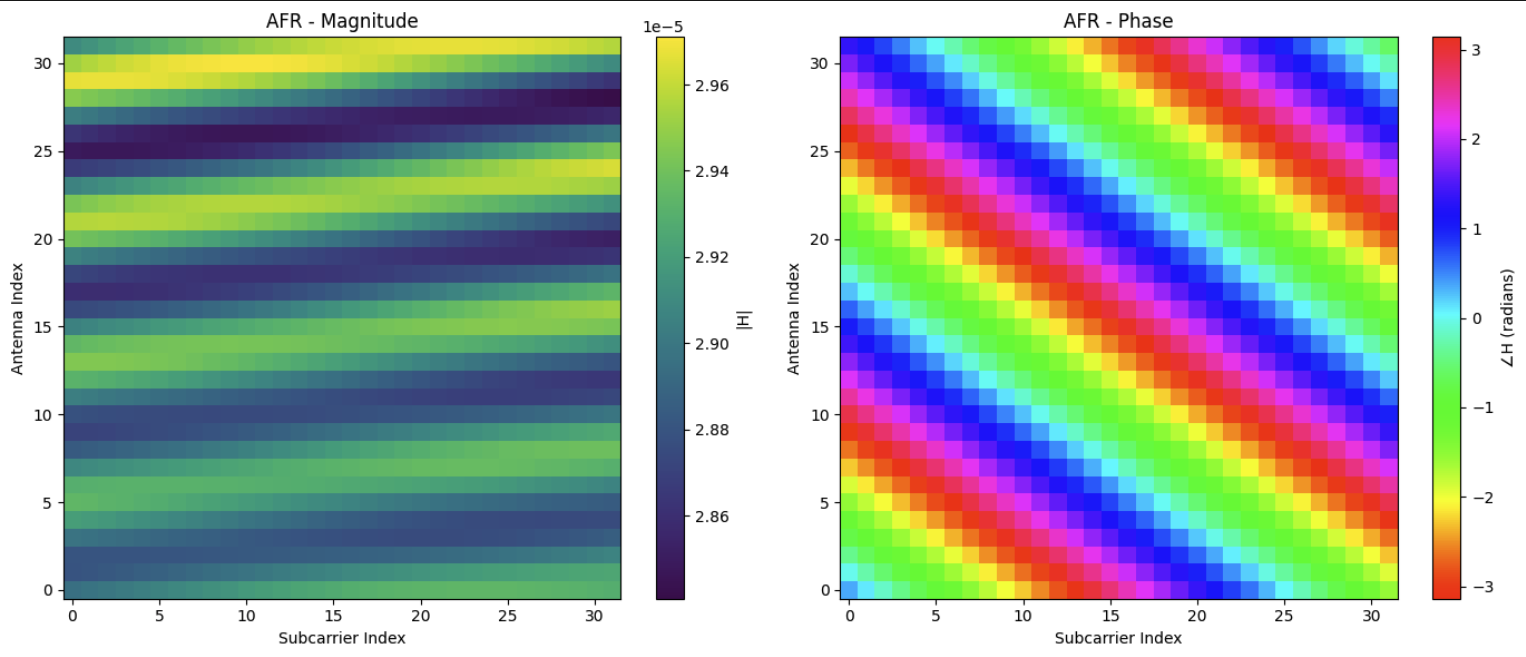
\includegraphics[width=0.9\linewidth]{figures/boston_afr.png}
    \caption{TX antenna-frequency response (magnitude on the left, phase on the right)}
    \label{fig:afr}
\end{figure}

\subsection{Performance Optimizations}

\begin{itemize}
  \item \textbf{Synthetic Array}: Treats array as continuous aperture for faster computation.
  \item \textbf{Per-TX Solving}: Reduces complexity; enables large-scale generation.
  \item \textbf{TX Association Filtering}: Processes only associated users per TX.
  \item \textbf{Radio Map Pre-filtering}: Uses fewer samples (e.g., $10^6$) than detailed path solving (e.g., $10^7$) for efficient coverage estimation.
\end{itemize}

\clearpage
\section{Available Scenes}

We generated a number of scenes using \texttt{scenegen} tool. These scenes are included here.

\subsection{Boston Downtown}

\begin{figure}[h]
    \centering
    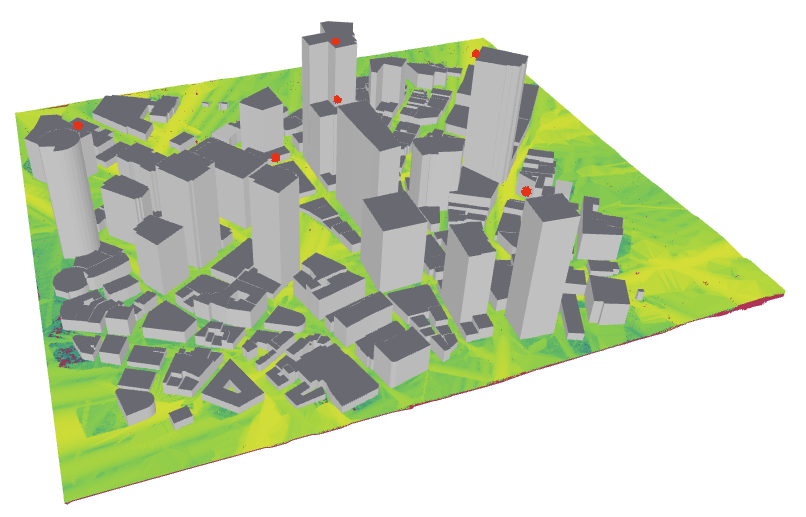
\includegraphics[width=0.5\linewidth]{figures/boston_1_cm.png}
    \caption{\texttt{boston\_1} scene}
\end{figure}

\subsection{Chicago Downtown}

\begin{figure}[h]
    \centering
    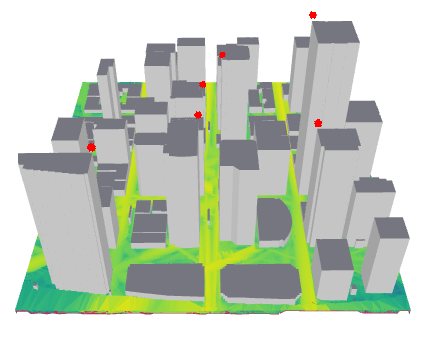
\includegraphics[width=0.5\linewidth]{figures/chicago_1_cm.png}
    \caption{\texttt{chicago\_1} scene}
\end{figure}

\clearpage

\subsection{New York City Manhattan}

\begin{figure}[h]
    \centering
    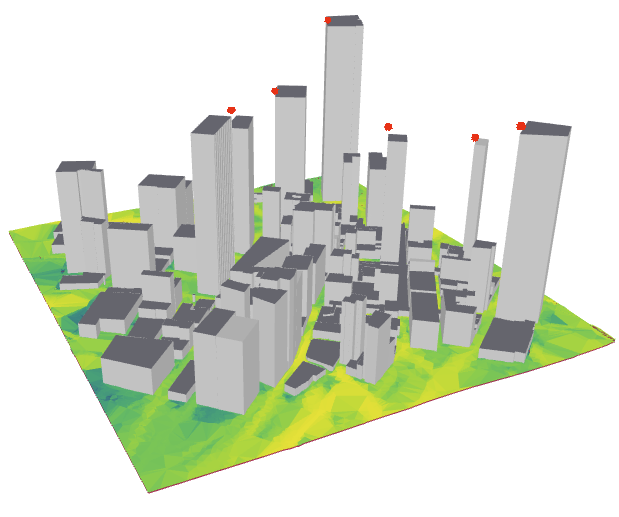
\includegraphics[width=0.5\linewidth]{figures/nyc_1_cm.png}
    \caption{\texttt{nyc\_1} scene}
\end{figure}

\subsection{San Francisco Downtown}

\begin{figure}[h]
    \centering
    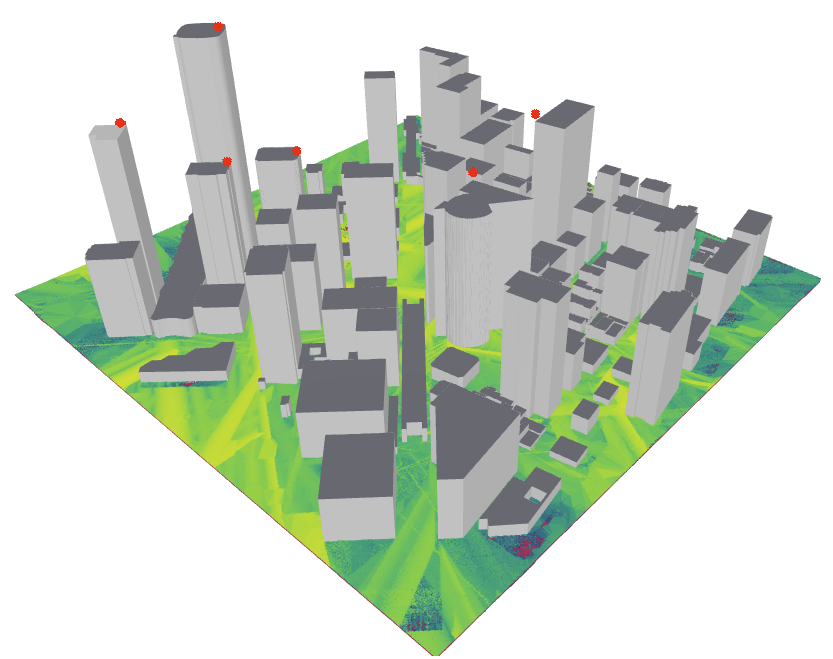
\includegraphics[width=0.5\linewidth]{figures/sf_1_cm.png}
    \caption{\texttt{sf\_1} scene}
\end{figure}

\subsection{Los Angeles Downtown}

\begin{figure}[h]
    \centering
    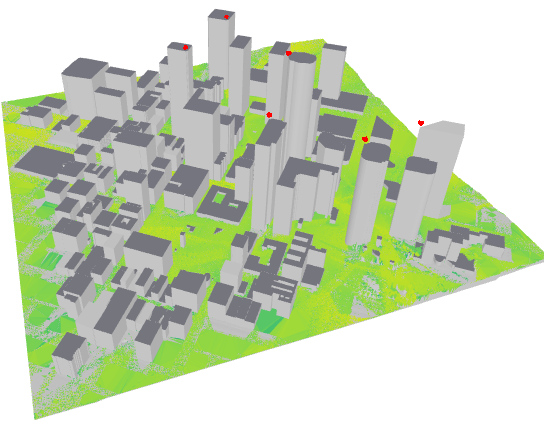
\includegraphics[width=0.5\linewidth]{figures/la_1_cm.png}
    \caption{\texttt{la\_1} scene}
\end{figure}

\end{document}